
\documentclass[letterpaper,hide notes,xcolor={table,svgnames},pdftex,10pt]{beamer}
\def\showexamples{t}


%\usepackage[svgnames]{xcolor}

%% Demo talk
%\documentclass[letterpaper,notes=show]{beamer}

\usecolortheme{crane}
\setbeamertemplate{navigation symbols}{}

\usetheme{MyPittsburgh}
%\usetheme{Frankfurt}

%\usepackage{tipa}

\usepackage{hyperref}
\usepackage{graphicx,xspace}
\usepackage[normalem]{ulem}

\newcommand\SF[1]{$\bigstar$\footnote{SF: #1}}

\usepackage[default]{sourcesanspro}
\usepackage[T1]{fontenc}

\newcounter{tmpnumSlide}
\newcounter{tmpnumNote}

% old question code
%\newcommand\question[1]{{$\bigstar$ \small \onlySlide{2}{#1}}}
% \newcommand\nquestion[1]{\ifdefined \presentationonly \textcircled{?} \fi \note{\par{\Large \textbf{?}} #1}}
% \newcommand\nanswer[1]{\note{\par{\Large \textbf{A}} #1}}


 \newcommand\mnote[1]{%
   \addtocounter{tmpnumSlide}{1}
   \ifdefined\showcues {~\tiny\fbox{\arabic{tmpnumSlide}}}\fi
   \note{\setlength{\parskip}{1ex}\addtocounter{tmpnumNote}{1}\textbf{\Large \arabic{tmpnumNote}:} {#1\par}}}

\newcommand\mmnote[1]{\note{\setlength{\parskip}{1ex}#1\par}}

%\newcommand\mnote[2][]{\ifdefined\handoutwithnotes {~\tiny\fbox{#1}}\fi
% \note{\setlength{\parskip}{1ex}\textbf{\Large #1:} #2\par}}

%\newcommand\mnote[2][]{{\tiny\fbox{#1}} \note{\setlength{\parskip}{1ex}\textbf{\Large #1:} #2\par}}

\newcommand\mquestion[2]{{~\color{red}\fbox{?}}\note{\setlength{\parskip}{1ex}\par{\Large \textbf{?}} #1} \note{\setlength{\parskip}{1ex}\par{\Large \textbf{A}} #2\par}\ifdefined \presentationonly \pause \fi}

\newcommand\blackboard[1]{%
\ifdefined   \showblackboard
  {#1}
  \else {\begin{center} \fbox{\colorbox{blue!30}{%
         \begin{minipage}{.95\linewidth}%
           \hspace{\stretch{1}} Some space intentionally left blank; done at the blackboard.%
         \end{minipage}}}\end{center}}%
         \fi%
}



%\newcommand\q{\tikz \node[thick,color=black,shape=circle]{?};}
%\newcommand\q{\ifdefined \presentationonly \textcircled{?} \fi}

\usepackage{listings}
\lstset{%
  keywordstyle=\bfseries,
  aboveskip=15pt,
  belowskip=15pt,
  captionpos=b,
  identifierstyle=\ttfamily,
  escapeinside={(*@}{@*)},
  stringstyle=\ttfamiliy,
  frame=lines,
  numbers=left, basicstyle=\scriptsize, numberstyle=\tiny, stepnumber=0, numbersep=2pt}

\usepackage{siunitx}
\newcommand\sius[1]{\num[group-separator = {,}]{#1}\si{\micro\second}}
\newcommand\sims[1]{\num[group-separator = {,}]{#1}\si{\milli\second}}
\newcommand\sins[1]{\num[group-separator = {,}]{#1}\si{\nano\second}}
\sisetup{group-separator = {,}, group-digits = true}

%% -------------------- tikz --------------------
\usepackage{tikz}
\usetikzlibrary{positioning}
\usetikzlibrary{arrows,backgrounds,automata,decorations.shapes,decorations.pathmorphing,decorations.markings,decorations.text}

\tikzstyle{place}=[circle,draw=blue!50,fill=blue!20,thick, inner sep=0pt,minimum size=6mm]
\tikzstyle{transition}=[rectangle,draw=black!50,fill=black!20,thick, inner sep=0pt,minimum size=4mm]

\tikzstyle{block}=[rectangle,draw=black, thick, inner sep=5pt]
\tikzstyle{bullet}=[circle,draw=black, fill=black, thin, inner sep=2pt]

\tikzstyle{pre}=[<-,shorten <=1pt,>=stealth',semithick]
\tikzstyle{post}=[->,shorten >=1pt,>=stealth',semithick]
\tikzstyle{bi}=[<->,shorten >=1pt,shorten <=1pt, >=stealth',semithick]

\tikzstyle{mut}=[-,>=stealth',semithick]

\tikzstyle{treereset}=[dashed,->, shorten >=1pt,>=stealth',thin]

\usepackage{ifmtarg}
\usepackage{xifthen}
\makeatletter
% new counter to now which frame it is within the sequence
\newcounter{multiframecounter}
% initialize buffer for previously used frame title
\gdef\lastframetitle{\textit{undefined}}
% new environment for a multi-frame
\newenvironment{multiframe}[1][]{%
\ifthenelse{\isempty{#1}}{%
% if no frame title was set via optional parameter,
% only increase sequence counter by 1
\addtocounter{multiframecounter}{1}%
}{%
% new frame title has been provided, thus
% reset sequence counter to 1 and buffer frame title for later use
\setcounter{multiframecounter}{1}%
\gdef\lastframetitle{#1}%
}%
% start conventional frame environment and
% automatically set frame title followed by sequence counter
\begin{frame}%
\frametitle{\lastframetitle~{\normalfont(\arabic{multiframecounter})}}%
}{%
\end{frame}%
}
\makeatother

\makeatletter
\newdimen\tu@tmpa%
\newdimen\ydiffl%
\newdimen\xdiffl%
\newcommand\ydiff[2]{%
    \coordinate (tmpnamea) at (#1);%
    \coordinate (tmpnameb) at (#2);%
    \pgfextracty{\tu@tmpa}{\pgfpointanchor{tmpnamea}{center}}%
    \pgfextracty{\ydiffl}{\pgfpointanchor{tmpnameb}{center}}%
    \advance\ydiffl by -\tu@tmpa%
}
\newcommand\xdiff[2]{%
    \coordinate (tmpnamea) at (#1);%
    \coordinate (tmpnameb) at (#2);%
    \pgfextractx{\tu@tmpa}{\pgfpointanchor{tmpnamea}{center}}%
    \pgfextractx{\xdiffl}{\pgfpointanchor{tmpnameb}{center}}%
    \advance\xdiffl by -\tu@tmpa%
}
\makeatother
\newcommand{\copyrightbox}[3][r]{%
\begin{tikzpicture}%
\node[inner sep=0pt,minimum size=2em](ciimage){#2};
\usefont{OT1}{phv}{n}{n}\fontsize{4}{4}\selectfont
\ydiff{ciimage.south}{ciimage.north}
\xdiff{ciimage.west}{ciimage.east}
\ifthenelse{\equal{#1}{r}}{%
\node[inner sep=0pt,right=1ex of ciimage.south east,anchor=north west,rotate=90]%
{\raggedleft\color{black!50}\parbox{\the\ydiffl}{\raggedright{}#3}};%
}{%
\ifthenelse{\equal{#1}{l}}{%
\node[inner sep=0pt,right=1ex of ciimage.south west,anchor=south west,rotate=90]%
{\raggedleft\color{black!50}\parbox{\the\ydiffl}{\raggedright{}#3}};%
}{%
\node[inner sep=0pt,below=1ex of ciimage.south west,anchor=north west]%
{\raggedleft\color{black!50}\parbox{\the\xdiffl}{\raggedright{}#3}};%
}
}
\end{tikzpicture}
}


%% --------------------

%\usepackage[excludeor]{everyhook}
%\PushPreHook{par}{\setbox0=\lastbox\llap{MUH}}\box0}

%\vspace*{\stretch{1}

%\setbox0=\lastbox \llap{\textbullet\enskip}\box0}

\setlength{\parskip}{\fill}

\newcommand\noskips{\setlength{\parskip}{1ex}}
\newcommand\doskips{\setlength{\parskip}{\fill}}

\newcommand\xx{\par\vspace*{\stretch{1}}\par}
\newcommand\xxs{\par\vspace*{2ex}\par}
\newcommand\tuple[1]{\langle #1 \rangle}
\newcommand\code[1]{{\sf \footnotesize #1}}
\newcommand\ex[1]{\uline{Example:} \ifdefined \presentationonly \pause \fi
  \ifdefined\showexamples#1\xspace\else{\uline{\hspace*{2cm}}}\fi}

\newcommand\ceil[1]{\lceil #1 \rceil}


\AtBeginSection[]
{
   \begin{frame}
       \frametitle{Outline}
       \tableofcontents[currentsection]
   \end{frame}
}



\pgfdeclarelayer{edgelayer}
\pgfdeclarelayer{nodelayer}
\pgfsetlayers{edgelayer,nodelayer,main}

\tikzstyle{none}=[inner sep=0pt]
\tikzstyle{rn}=[circle,fill=Red,draw=Black,line width=0.8 pt]
\tikzstyle{gn}=[circle,fill=Lime,draw=Black,line width=0.8 pt]
\tikzstyle{yn}=[circle,fill=Yellow,draw=Black,line width=0.8 pt]
\tikzstyle{empty}=[circle,fill=White,draw=Black]
\tikzstyle{bw} = [rectangle, draw, fill=blue!20, 
    text width=4em, text centered, rounded corners, minimum height=2em]
    
    \newcommand{\CcNote}[1]{% longname
	This work is licensed under the \textit{Creative Commons #1 3.0 License}.%
}
\newcommand{\CcImageBy}[1]{%
	\includegraphics[scale=#1]{creative_commons/cc_by_30.pdf}%
}
\newcommand{\CcImageSa}[1]{%
	\includegraphics[scale=#1]{creative_commons/cc_sa_30.pdf}%
}
\newcommand{\CcImageNc}[1]{%
	\includegraphics[scale=#1]{creative_commons/cc_nc_30.pdf}%
}
\newcommand{\CcGroupBySa}[2]{% zoom, gap
	\CcImageBy{#1}\hspace*{#2}\CcImageNc{#1}\hspace*{#2}\CcImageSa{#1}%
}
\newcommand{\CcLongnameByNcSa}{Attribution-NonCommercial-ShareAlike}

\newenvironment{changemargin}[1]{% 
  \begin{list}{}{% 
    \setlength{\topsep}{0pt}% 
    \setlength{\leftmargin}{#1}% 
    \setlength{\rightmargin}{1em}
    \setlength{\listparindent}{\parindent}% 
    \setlength{\itemindent}{\parindent}% 
    \setlength{\parsep}{\parskip}% 
  }% 
  \item[]}{\end{list}} 




\title{Lecture 14 --- Classical Synchronization Problems }

\author{Jeff Zarnett \\ \small \texttt{jzarnett@uwaterloo.ca}}
\institute{Department of Electrical and Computer Engineering \\
  University of Waterloo}
\date{\today}


\begin{document}

\begin{frame}
  \titlepage

 \end{frame}

\begin{frame}
\frametitle{Classical Problems}

Various operating systems textbooks provide a few ``classical problems''. 

Scenarios phrased in real-world terms; an analogy for OS problems. 

Used to test any newly-proposed synchronization or coordination scheme.

 The solutions make use of semaphores as the basis for mutual exclusion. 
 
 We are going to examine three of them: 
 \begin{itemize}
 \item The producer-consumer problem 
 \item The readers-writers problem 
 \item The dining philosophers problem.
 \end{itemize}


\end{frame}


\begin{frame}
\frametitle{Producer-Consumer Problem}

Most common: producer-consumer problem (bounded-buffer-problem). 

Two processes share a common buffer that is of fixed size. 

One process is the producer: it generates data and puts it in the buffer.

The other is the consumer: it takes data out of the buffer. 

This problem can be generalized to have $p$ producers and $c$ consumers.

\end{frame}



\begin{frame}
\frametitle{Producer-Consumer Rules}
It is not possible to write into a buffer that is already full. 

It is similarly not possible to read from an empty buffer.

 Either situation can block a process. 

\end{frame}

\begin{frame}
\frametitle{Producer-Consumer Problem}

To keep track of the number of items in the buffer, we have a variable \texttt{count}.

  This is a variable shared between more than one thread. 
  
Therefore access to this should be controlled with mutual exclusion. 

The maximum number of elements in the buffer is defined as \texttt{BUFFER\_SIZE}.


\end{frame}


\begin{frame}[fragile]
\frametitle{Producer-Consumer Solution 1}

If busy-waiting is permitted we can get away with one mutex.


\begin{multicols}{2}
\textbf{Producer}
  \begin{verbatim}
	 1. [produce item]
	 2. added = false
	 3. while added is false
	 4.    wait( mutex )
	 5.    if count < BUFFER_SIZE
	 6.        [add item to buffer]
	 7.        count++
	 8.        added = true
	 9.    end if
	10.    signal( mutex )
	11. end while
  \end{verbatim}
\columnbreak
\textbf{Consumer}
  \begin{verbatim}
	 1. removed = false
	 2. while removed is false
	 3.    wait( mutex )
	 4.    if count > 0
	 5.      [remove item from buffer]
	 6.      count--
	 7.      removed = true
	 8.    end if
	 9.    signal( mutex )
	10. end while
	11. [consume item]
  \end{verbatim}
\end{multicols}
\vspace{-2em}

\end{frame}



\begin{frame}
\frametitle{Producer-Consumer Solution 1 Analysis}

While this accomplishes what we want, it is inefficient. 

Let's add a third rule that says we want to avoid busy-waiting.

Thus, when the producer is waiting for space it will be blocked.

Same for the consumer when waiting for an element. 
\end{frame}



\begin{frame}
\frametitle{Producer-Consumer Solution 2}

To accomplish this, we will need two general semaphores, each with maximum value of \texttt{BUFFER\_SIZE}. 

The first is called \texttt{items}:\\
\quad It starts at 0 and represents how many spaces in the buffer are full. 

The second is the mirror image \texttt{spaces};\\
\quad It starts at \texttt{BUFFER\_SIZE} and represents the number of empty spaces.


\end{frame}



\begin{frame}[fragile]
\frametitle{Producer-Consumer Solution 2}

\begin{multicols}{2}
\textbf{Producer}
  \begin{verbatim}
	 1. [produce item]
	 2. wait( spaces )
	 3. [add item to buffer]
	 4. signal( items )
  \end{verbatim}
\columnbreak
\textbf{Consumer}
  \begin{verbatim}
	 1. wait( items )
	 2. [remove item from buffer]
	 3. signal( spaces )
	 4. [consume item]
  \end{verbatim}
\end{multicols}
\vspace{-2em}

\end{frame}


\begin{frame}
\frametitle{Producer-Consumer Solution 2 Analysis}

The producer can continue to produce items until the buffer is full and the consumer can continue to consume items until the buffer is empty. 

This solution works okay, given two assumptions:

(1) Adding an item to the buffer and removing an item from the buffer add to and remove from the ``next'' space.


(2) There is exactly one producer and one consumer in the system. 

\end{frame}



\begin{frame}[fragile]
\frametitle{General Producer-Consumer Solution}

Now let us allow for multiple producers and multiple consumers.

\begin{multicols}{2}
\textbf{Producer}
  \begin{verbatim}
	 1. [produce item]
	 2. wait( spaces )
	 3. wait( mutex )
	 4. [add item to buffer]
	 5. signal( mutex )
	 6. signal( items )
  \end{verbatim}
\columnbreak
\textbf{Consumer}
  \begin{verbatim}
	 1. wait( items )
	 2. wait( mutex )
	 3. [remove item from buffer]
	 4. signal( mutex )
	 5. signal( spaces )
	 6. [consume item]
  \end{verbatim}
\end{multicols}


\end{frame}



\begin{frame}
\frametitle{General Producer-Consumer Analysis}

This situation should be setting off some alarm bells in your mind. 

Recall the possibility of deadlock: all threads getting stuck.

The hint that we might have a problem is one \texttt{wait} statement inside another.

Seeing this pattern is not a guarantee that deadlock is going to happen.

We must analyze the code to determine if there is a problem. 


\end{frame}



\begin{frame}
\frametitle{Checking for a Deadlock}

You should be able to reason that this solution will not get stuck.

 You may choose a strategy along the lines of ``proof by contradiction'' and try to come up with a scenario that leads to deadlock. 
 
 If you are unable to find one, then you may have a suitable solution.\\
 \quad Mind you, someone else may be able to...
 
 This is not a substitute for a formal mathematical proof, but the logic in your analysis should be convincing.
\end{frame}



\begin{frame}[fragile]
\frametitle{General Producer-Consumer Solution 2}

Consider this alternate solution:

\begin{multicols}{2}
\textbf{Producer}
  \begin{verbatim}
	 1. [produce item]
	 2. wait( mutex )
	 3. wait( spaces )
	 4. [add item to buffer]
	 5. signal( items )
	 6. signal( mutex )
  \end{verbatim}
\columnbreak
\textbf{Consumer}
  \begin{verbatim}
	 1. wait( mutex )
	 2. wait( items )
	 3. [remove item from buffer]
	 4. signal( spaces )
	 5. signal( mutex )
	 6. [consume item]
  \end{verbatim}
\end{multicols}

\end{frame}



\begin{frame}
\frametitle{General Producer-Consumer Solution 2 Analysis}

We have swapped the order of the \texttt{wait} statements. 

As before, we need to analyze this code to determine if there is a problem. 

This solution does have the deadlock problem. 

Try to think of a scenario where that happens.

\end{frame}



\begin{frame}
\frametitle{General Producer-Consumer Solution 2 Analysis}

Start of execution, when the buffer is empty: the consumer thread runs first. 

It will wait on \texttt{mutex}, be allowed to proceed, and then will be blocked on \texttt{items} because the buffer is initially empty. 

When the producer thread runs, it waits on \texttt{mutex} and cannot proceed because the consumer thread is in the critical section there. 

So the producer is blocked and can never produce any items. Deadlock!

This situation could occur any time the buffer is empty.

\end{frame}



\begin{frame}
\frametitle{Deadlock}
If the above code were implemented it is not a certainty that there will be a deadlock every time.

 In fact, the code will probably work fine most of the time. 
 
If we have found one scenario that can lead to deadlock, there is no need to look for other failure cases.
 
 We can write off this solution and replace it with a better one.

\end{frame}



\begin{frame}
\frametitle{The Readers-Writers Problem}

Concurrent reading \& modification of a data structure or record by $>1$ thread. 

A writer will modify the data; a reader will read it only without modification. 

Unlike the producer-consumer problem, some concurrency is allowed:

\begin{enumerate}
\item Any number of readers may be in the critical section simultaneously.
\item Only one writer may be in the critical section (and when it is, no readers)
\end{enumerate}


\end{frame}



\begin{frame}
\frametitle{The Readers-Writers Problem}

A writer cannot enter the critical section while any other thread is there. 

While a writer is in the critical section, neither readers nor writers may enter. 

This is very often how file systems work.

If any thread could read or write the shared data structure, we would have to use the general mutual exclusion solution. 

The general mutual exclusion routine would prevent errors, but is a serious performance reduction.

\end{frame}



\begin{frame}
\frametitle{Readers-Writers Solution 1}
Let us keep track of the number of readers at any given time with \texttt{readers}. 

We will need a way of protecting this variable from concurrent modifications, so there will have to be a binary semaphore \texttt{mutex}. 

We will also need one further semaphore, \texttt{roomEmpty}.

A writer has to wait for the room to be empty (i.e., \texttt{wait} on the \texttt{roomEmpty} semaphore) before it can enter.
\end{frame}



\begin{frame}[fragile]
\frametitle{Readers-Writers Solution 1}

\begin{multicols}{2}
\textbf{Writer}
  \begin{verbatim}
	 1. wait( roomEmpty )
	 2. [write data]
	 3. signal( roomEmpty )
	 
	 
	 
	 
	 
	 
	 
	 
	 
	 
  \end{verbatim}
\columnbreak
\textbf{Reader}
  \begin{verbatim}
	 1. wait( mutex )
	 2. readers++
	 3. if readers == 1
	 4.     wait( roomEmpty )
	 5. end if
	 6. signal( mutex )
	 7. [read data]
	 8. wait( mutex )
	 9. readers--
	10. if readers == 0
	11.     signal( roomEmpty )
	12. end if
	13. signal( mutex )
  \end{verbatim}
\end{multicols}
\vspace{-2em}

\end{frame}

\begin{frame}
\frametitle{Readers-Writers Solution 1 Analysis}

The first reader that arrives encounters the situation that the room is empty, so it ``locks'' the room (waiting on the \texttt{roomEmpty} semaphore).

That will prevent writers from entering the room. 

Additional readers do not check if the room is empty; they just proceed to enter. 

When the last reader leaves the room, it signals that the room is empty (``unlocking it'' to allow a writer in). 

This pattern is sometimes called the \alert{light switch}.

\end{frame}


\begin{frame}
\frametitle{Readers-Writers Solution 1 Analysis}

The reader code has that situation that makes us concerned.\\
\quad A wait on \texttt{roomEmpty} inside a critical section controlled by \texttt{mutex}. 

With a bit of reasoning, we can convince ourselves that there is no deadlock.

A reader waits on \texttt{roomEmpty} only if a writer is currently in its critical section.

As long as the write operation takes finite time, eventually the writer will signal the \texttt{roomEmpty} semaphore and the threads can continue. 

Deadlock is not a problem.

\end{frame}


\begin{frame}
\frametitle{Readers-Writers Solution 1 Analysis}

There is, however, a second problem that we need to be concerned about. 

Suppose some readers are in the room, and a writer arrives. 

The writer must wait until all the readers have left the room. 

When each of the readers is finished, it exits the room. 

In the meantime, more readers arrive and enter the room.
\end{frame}


\begin{frame}
\frametitle{Readers-Writers Solution 1 Analysis}

So even though each reader is in the room for only a finite amount of time, there is never a moment when the room has no readers in it. 

This undesirable situation is not deadlock, because the reader threads are not stuck, but the writer (and any subsequent writers) is (are) going to wait forever.

This is a situation called \alert{starvation}: a thread never gets a chance to run.


\end{frame}


\begin{frame}
\frametitle{Starvation}

Recall criterion 3 of properties we want in any mutual exclusion solution:\\
\quad It must not be possible for a thread to be delayed indefinitely. 

This problem is just as bad as deadlock in that if it is discovered, it eliminates a proposed solution as an acceptable option.

Even though starvation might only be an unlikely event. 

We must therefore improve on this solution such that there is no longer the possibility that a writer starves.


\end{frame}


\begin{frame}
\frametitle{Readers-Writers Solution 2}

When a writer arrives, any readers should be permitted to finish their read.\\
\quad No new readers should be allowed to start reading. 

Eventually, all the readers currently in the critical section will finish. 

The writer will get a turn, because the room is empty.

When the writer is done, all the readers that arrived after the writer will be able to enter.

\end{frame}


\begin{frame}[fragile]
\frametitle{Readers-Writers Solution 2}
\begin{multicols}{2}
\textbf{Writer}
  \begin{verbatim}
	 1. wait( turnstile )
	 2. wait( roomEmpty )
	 3. [write data]
	 4. signal( turnstile )
	 5. signal( roomEmpty )
	 
	 
	 
	 
	 
	 
	 
	 
	 
	 
  \end{verbatim}
\columnbreak
\textbf{Reader}
  \begin{verbatim}
	 1. wait( turnstile )
	 2. signal( turnstile )
	 3. wait( mutex )
	 4. readers++
	 5. if readers == 1
	 6.     wait( roomEmpty )
	 7. end if
	 8. signal( mutex )
	 9. [read data]
	10. wait( mutex )
	11. readers--
	12. if readers == 0
	13.     signal( roomEmpty )
	14. end if
	15. signal( mutex )
  \end{verbatim}
\end{multicols}

\end{frame}


\begin{frame}
\frametitle{Readers-Writers Solution 2 Analysis}

Does this solution satisfy our goals of avoidance of deadlock and starvation? 

Starvation is fairly easy to assess: the first attempt at the solution had one scenario leading to starvation and this solution addresses it. 

You should be able to convince yourself that the solution as described cannot starve the writers or readers.


\end{frame}


\begin{frame}
\frametitle{Readers-Writers Solution 2 Analysis}

On to deadlock: the reader code is minimally changed from before 

The writer has that dangerous pattern: two waits. 

If the writer is blocked on the \texttt{roomEmpty} semaphore, no readers or writers could advance past the turnstile and no writers. 

If the writer is blocked on that semaphore, there are readers in the room. 

The readers will individually finish and leave (their progress is not impeded). 

So the room will eventually become empty; the writer will be unblocked.


\end{frame}

\begin{frame}
\frametitle{Readers-Writers Solution 2 Analysis}

Note that this solution does not give writers any particular priority: when a writer exits it signals \texttt{turnstile} and that may unblock a reader or a writer. 

If it unblocks a reader, a whole bunch of readers may enter before the next writer is unblocked and locks the turnstile again. 

That may or may not be desirable, depending on the application. 

In any event, it does mean it is possible for readers to proceed even if a writer is queued. 

If there is a need to give writers priority, there are techniques for doing so.\\
\quad But we will not examine them here.

\end{frame}

\begin{frame}
\frametitle{The Dining Philosophers Problem}

The dining philosophers problem was also proposed by Dijkstra in 1965. 

The problem can have $n$ philosophers, but problem is typically described as 5. 

 These five smart individuals spend their lives thinking, but every so often, they need to eat. They share a table, each having his or her own chair. 
 
In the centre of the table is a bowl of rice, \& it is laid with 5 single chopsticks. 

\end{frame}

\begin{frame}
\frametitle{The Dining Philosophers Problem}

\begin{center}
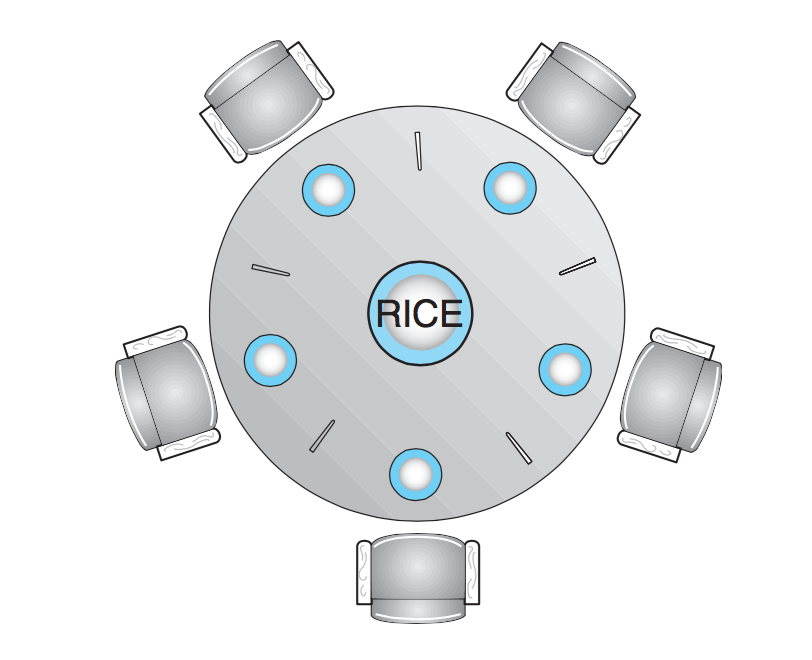
\includegraphics[width=0.6\textwidth]{images/philosopher-table.png}
\end{center}

\end{frame}

\begin{frame}
\frametitle{Dinner Time}

When a philosopher wishes to eat, she sits down at her designated chair, and attempts to pick up the two chopsticks that are nearest. 

Philosophers are polite and therefore do not grab a chopstick out of the hands of a colleague.

 When a philosopher has both chopsticks, she may eat rice, and when she is finished, she puts down the chopsticks and goes back to thinking.


\end{frame}

\begin{frame}
\frametitle{Dining with Semaphores}

 Suppose then that semaphores are the method for managing things. 
 
 Because only one person can be in possession of a chopstick at a time, each chopstick may be represented by a binary semaphore. 
 
When the philosopher sits down he attempts to acquire the left chopstick, then the right, eats, and puts the chopsticks down. 
 
This works fine, until all philosophers sit down at the same time. Each grabs the chopstick to his or her left.

 None of them are able to acquire the chopstick to his or her right (because someone has already picked it up). 
 
 None of the philosophers can eat; they are all stuck. Deadlock.

\end{frame}

\begin{frame}
\frametitle{Deadlock at the Dinner Table}

This example makes it more clear why we call a situation where a thread never gets to run ``starvation''. 

If a philosopher is never able to get both chopsticks, that philosopher will never be able to eat.

Though I am not an expert on biology, I have it on good authority that people who do not eat anything end up eventually starving to death. 

Even philosophers.

\end{frame}

\begin{frame}
\frametitle{Saving the Philosophers}

One thing that would guarantee that this problem does not occur is to protect the table with a binary semaphore. 

This would allow exactly one philosopher at a time to eat, but at the very least, deadlock and starvation would be avoided. 

Although this works, it is a suboptimal solution. 

There are five seats and five chopsticks. Yet only one person is eating at a time. 

\end{frame}


\begin{frame}
\frametitle{No, the Pigeons are not for Eating}

What if we limit the number of philosophers at the table concurrently to four? 

The pigeonhole principle applies here: if there are $k$ pigeonholes and more than $k$ pigeons, at least one pigeonhole must have at least two pigeons. 

Thus, at least one of the four philosophers can get two chopsticks. 

Implementation is easy: a general semaphore with a max and initial value of 4.

\end{frame}

\begin{frame}
\frametitle{Invite a Leftie}

The problem above occurs because every philosopher tries to pick up the left chopstick first. 

If some of them try to pick up the left and some pick up the right first, then deadlock will not happen.

This problem is a great basis to launch into a discussion about deadlock...

\end{frame}


\end{document}

